%%%%%%%%%%%%%%%%%%%%%%%%%%%%%%%
\documentclass{beamer}
\usepackage[T1]{fontenc}
\usepackage[light,math]{iwona}
\usetheme[pageofpages=of,	% String used between current page & total page count.
   	alternativetitlepage=true,	% Use the fancy title page.
      	titlepagelogo=logoCGU,	% Logo for the first page.
       	watermark=logoCGU_45cut,	% Watermark used in every page.
      	watermarkheight=50px,	% Height of the watermark.
       	watermarkheightmult=4,	% 4 times bigger than watermarkheight.
]{Claremont}

%%%%%%%%%%%%%%%%%%%%%%%%%%%%%%%
\usepackage{graphicx}
\graphicspath{{./figs/}} % graphic files in "figs"
\usepackage{caption}
\usepackage{subcaption}
\usepackage{animate}
\usepackage{animfp}
\usepackage{setspace}
%\singlespacing
%\onehalfspacing
%\double spacing
\setstretch{1.25}
%%%%%%%%%%%%%%%%%%%%%%%%%%%%%%%

%%%%%%Get source code listings nicely printed%%%%%%
\usepackage{listings}
\usepackage{color}
\usepackage{textcomp}
\lstset{
	backgroundcolor=\color{black},  	
	rulecolor=,
	language=C++,				% the language of the code
        basicstyle=\scriptsize,		% the size of the fonts that are used for the code
        numbers=left,				% where to put the line-numbers
        numberstyle=\tiny,  			% the size of the fonts that are used for the line-numbers
        stepnumber=2,                   	% the step between two line-numbers
        numbersep=5pt,                  	% how far the line-numbers are from the code
        upquote=true,
        aboveskip={1.5\baselineskip},
        columns=fixed,
        showstringspaces=false,		% underline spaces within strings
        extendedchars=true,
        prebreak = \raisebox{0ex}[0ex][0ex]{\ensuremath{\hookleftarrow}},
        frame=single,
        tabsize=2,                      		% sets default tabsize to 2 spaces
        captionpos=b,                   		% sets the caption-position to bottom
        breaklines=true,                		% sets automatic line breaking
        breakatwhitespace=false,        	
        showtabs=false,
        showspaces=false,
        showstringspaces=false,
        identifierstyle=\ttfamily,
        keywordstyle=\color{magenta},
        ndkeywords={std, cout, cerr, cin, endl, is_open, setw, pow, exp, sqrt, fabs},
        ndkeywordstyle=\color{cyan},
        commentstyle=\color[rgb]{0.133,0.545,0.133},
        stringstyle=\color{red!75},
}
%%%%%%%%%%%%%%%%%%%%%%%%%%%%%%

%%%%%%%%%%%%%%%%%%%%%%%%%%%%%%
\title[Towards the Next Generation of High-Frequency Trading Models]{{\fontsize{12}{30} \textsc{Towards the Next Generation of High-Frequency Trading Models}}}

\author[Copyright \copyright Henry Schellhorn]{{\fontsize{10}{12}\textsc{Henry Schellhorn}} \qquad \qquad \qquad
	\qquad \qquad \qquad\qquad \qquad \qquad\qquad \qquad \qquad\qquad \qquad \qquad
	\and {\fontsize{8}{10}\textsc{With David German \& Thanh Hoang}}
	}
	
\institute[CGU]{{\fontsize{9}{10}
	\textsc{Claremont Graduate University}
}}
\date[March 27, 2013]{{\fontsize{8}{8}March 27, 2013}}
%%%%%%%%%%%%%%%%%%%%%%%%%%%%%%

%%%%%%%%%%%%%%%%%%%%%%%%%%%%%%
\begin{document}

% Page 1
\begin{frame}[plain, shrink=0]
	\titlepage
\end{frame}

% Page 2
\section{Outline}
\begin{frame}[shrink=20]{{\color{cyan}Outline}}
\bigskip

\begin{enumerate}

\item Option Pricing in a Liquid Market

\vspace{8pt}
\item Trading Limit Orders

\vspace{8pt}
\item Option Pricing in an Illiquid Market

\vspace{8pt}
\item Empirical Analysis

\end{enumerate}

\end{frame}

%%%%%%%%%%%%%%%%%%%%%%%%%%%%%%
% Section 1
\section{Option Pricing in a Liquid Market}

% Page 3
\begin{frame}[shrink=25]{{\color{cyan}Option Pricing in a Liquid Market}}
\bigskip
Model for Asset Price $\pi $ at time $t$
\begin{equation*}
	\pi (t,\omega )=\pi (0)\exp \left( \left(\mu -\frac{\sigma ^{2}}{2} \right) t+\sigma W(t,\omega) \right)
\end{equation*}
\qquad \qquad where:

\begin{description}
\item[] $\omega$: the state of the world ("scenario", "outcome"),

\item[] $\mu$: the \textit{drift},

\item[] $\sigma$: the \textit{volatility},

\item[] $W$: Brownian Motion.

\end{description}

\end{frame}

% Page 4
\begin{frame}[shrink=30]{{\color{cyan}{\large Option Pricing in a Liquid Market: what is Brownian Motion?}}}
\bigskip
Random walk: equal probability at each (discrete) time-step to go up or down.

\vspace{10pt}
\begin{figure}[H]
\begin{center}
	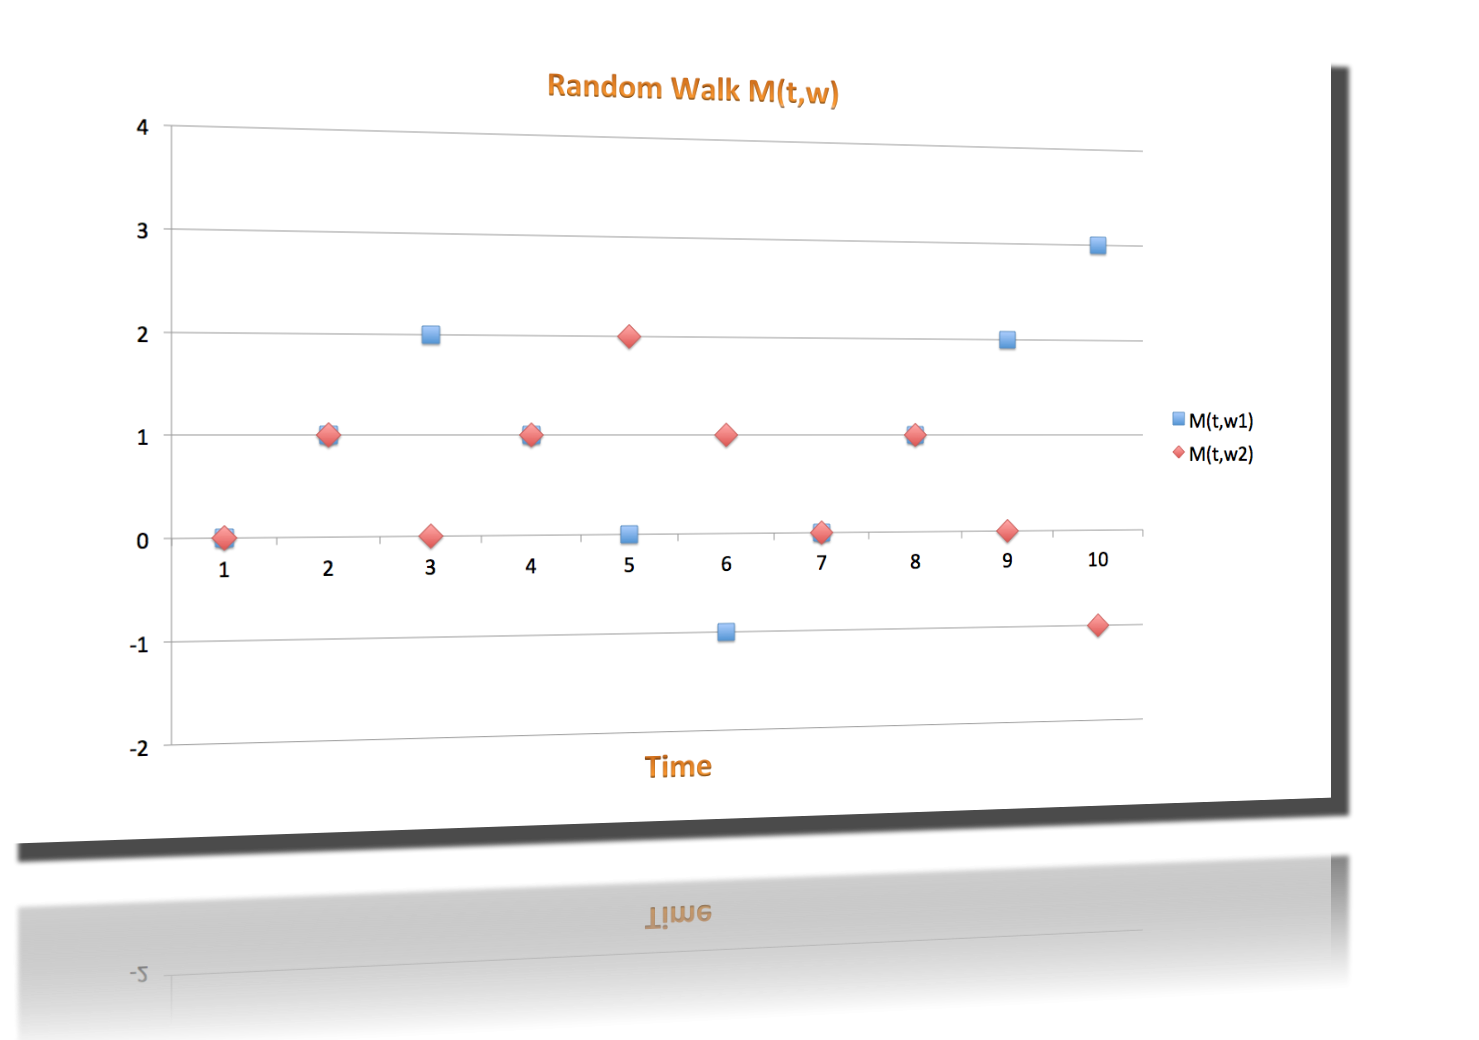
\includegraphics[height=0.8\textheight]{Random_Walk.png}
\caption{Random Walk.}
\label{fig:random_walk}
\end{center}
\end{figure}

\end{frame}

% Page 5
\begin{frame}[shrink=30]{{\color{cyan}{\large Option Pricing in a Liquid Market: what is Brownian Motion?}}}
\bigskip
Random walk: equal probability at each (discrete) time-step to go up or down.

\vspace{8pt}
Brownian Motion: accelerate time:
\vspace{10pt}
\begin{figure}[H]
\begin{center}
	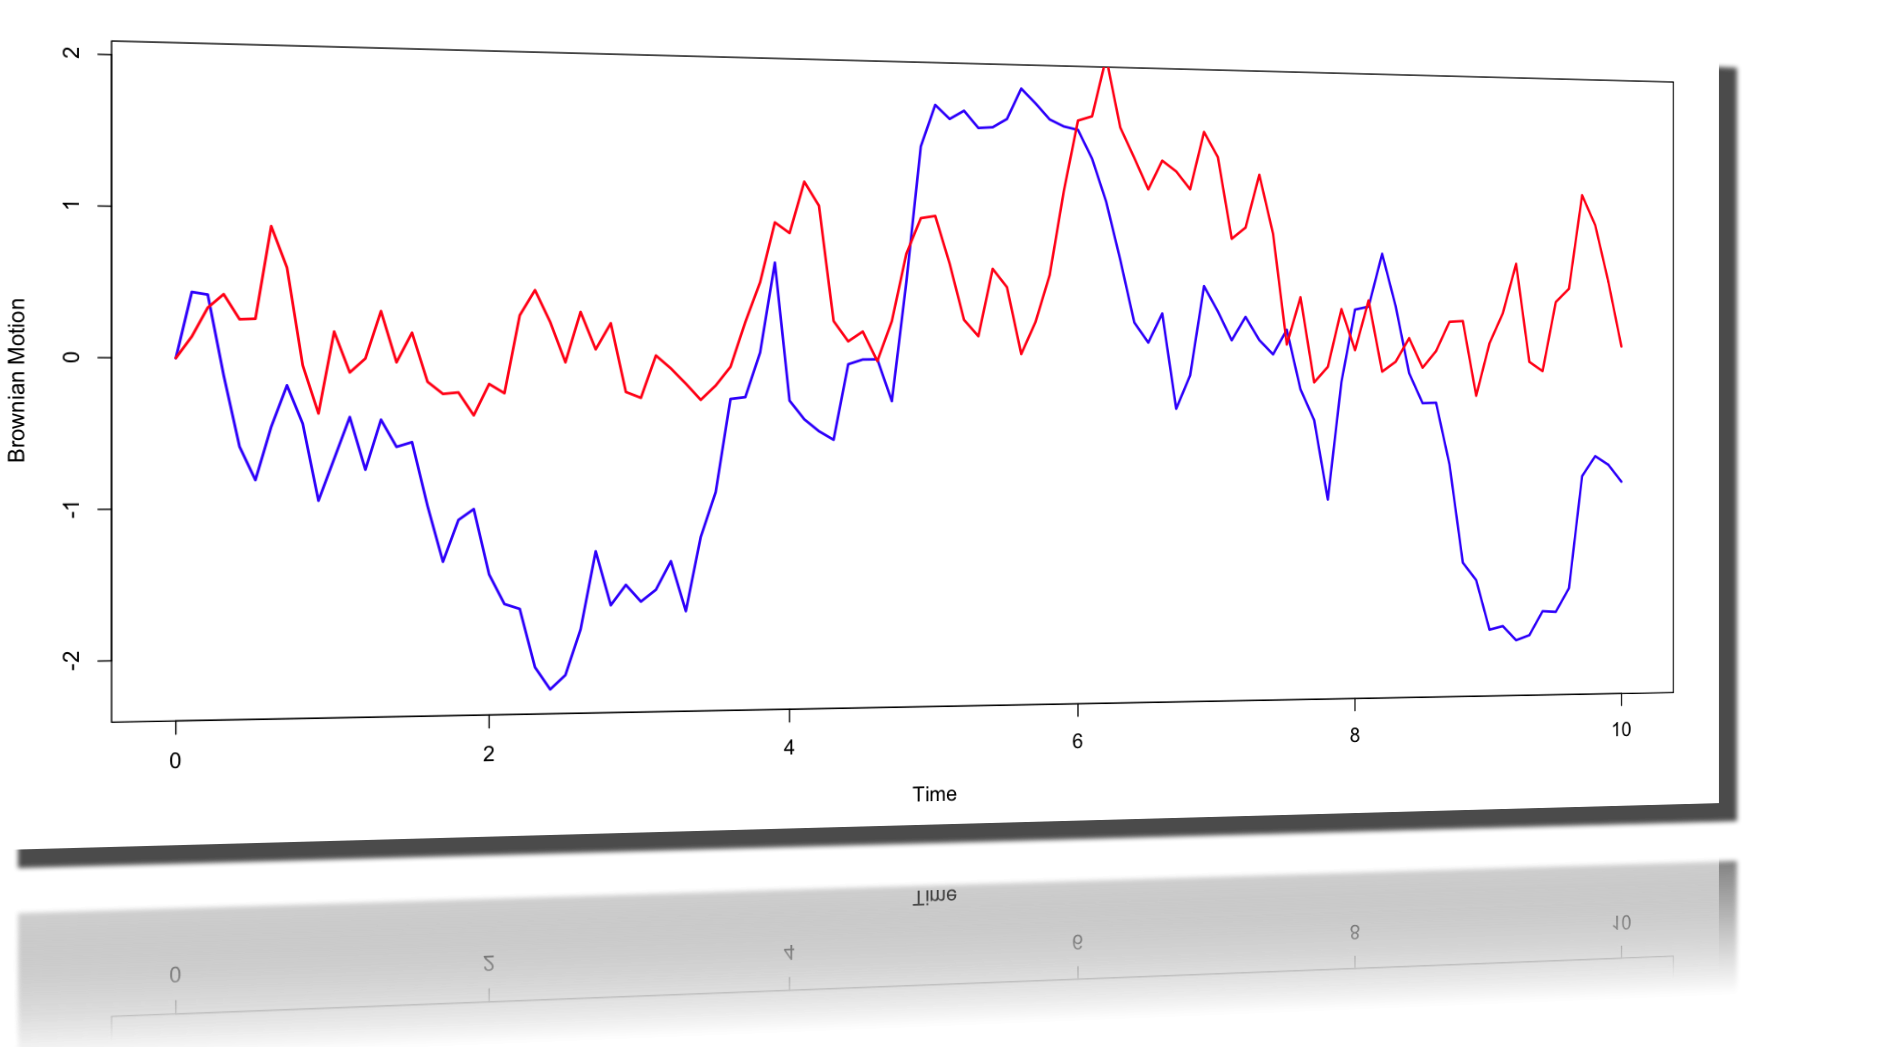
\includegraphics[height=0.8\textheight]{Brownian_Motion_2.png}
\caption{Brownian Motion.}
\label{fig:brownian_motion}
\end{center}
\end{figure}

\end{frame}

% Page 6
\begin{frame}[shrink=25]{{\color{cyan}{\large Option Pricing in a Liquid Market: Stochastic Calculus}}}
\bigskip

The Chain rule is different

\vspace{10pt}
\begin{itemize}
\item Regular calculus: with a differentiable path $x(t)$
\begin{equation*}
\frac{d}{dt}f(x(t),t)=\frac{\partial f}{\partial x}\frac{\partial x(t)}{\partial t}+\frac{\partial f}{\partial t}
\end{equation*}

\vspace{10pt}
\item Stochastic calculus: with a non-differentiable path $W(t)$
\begin{equation*}
df(W(t),t)=\frac{\partial f}{\partial x}dW(t)+\frac{1}{2}\frac{\partial^{2}f}{\partial^{2}x}dt+\frac{\partial f}{\partial t}dt
\end{equation*}
(Ito's lemma)
\end{itemize}

\end{frame}

% Page 7
\begin{frame}[shrink=38]{{\color{cyan}{\large Option Pricing in a Liquid Market: the Black-Scholes Formula}}}
\bigskip
\begin{block}{Call Option}
A call option is a contract which gives the owner the right to buy an (underlying)\ stock at a future time $T$ for a given \textit{strike price} $K$.
\end{block}

\begin{block}{Theorem}
If there is no arbitrage, the price of the call option at time zero is:
\vspace{-8pt}
\begin{equation*}
C(0)=E^{\mathbb{Q}}[\max (\pi (T)-K,0)]
\end{equation*}
\end{block}

{\color{magenta}\textbf{Observation:}} $\mathbb{Q}$ is called the \textit{risk-neutral} measure. It is by definition the measure where $\pi $ is a\textit{\ martingale}, i.e., where:
\vspace{-5pt}
\begin{equation*}
\pi (0)=E^{\mathbb{Q}}[\pi (t)]\text{ \ \ \ }\forall t>0
\end{equation*}

Equivalently, this is the measure where $W^{\mathbb{Q}}(t)\equiv W(t)+\frac{\mu }{\sigma }t$ is Brownian motion
\vspace{-5pt}
\begin{align*}
\pi (t) &=\pi (0)\exp \left( \left(\mu -\frac{\sigma ^{2}}{2} \right)t+\sigma W(t) \right) \\
	&=\pi (0)\exp \left(-\frac{\sigma ^{2}t}{2}+\sigma \left( W(t)+\frac{\mu }{\sigma }t \right) \right)\\
	&=\pi (0)\exp \left(-\frac{\sigma ^{2}t}{2}+\sigma W^{\mathbb{Q}}(t) \right)
\end{align*}

The drift $\mu $ disappears. The option price depends only on volatility $\sigma$!

\end{frame}

%%%%%%%%%%%%%%%%%%%%%%%%%%%%%%
% Section 2
\section{Trading Limit Orders}

% Page 8
\begin{frame}[shrink=25]{{\color{cyan}Market vs Limit Orders}}
\bigskip
A (buy) market order specifies
\vspace{5pt}
\begin{itemize}
\item how many shares a trader wants to buy,
\vspace{5pt}
\item that he is willing to buy them at any price.
\end{itemize}

\bigskip
A (buy) limit order specifies
\vspace{5pt}
\begin{itemize}
\item how many shares a trader wants to buy,
\vspace{5pt}
\item at what maximum price he is willing to buy them.
\end{itemize}

\end{frame}

% Page 9
\begin{frame}[shrink=30]{{\color{cyan}Limit order matching mechanism}}
\bigskip
\begin{figure}[H]
	\centering
	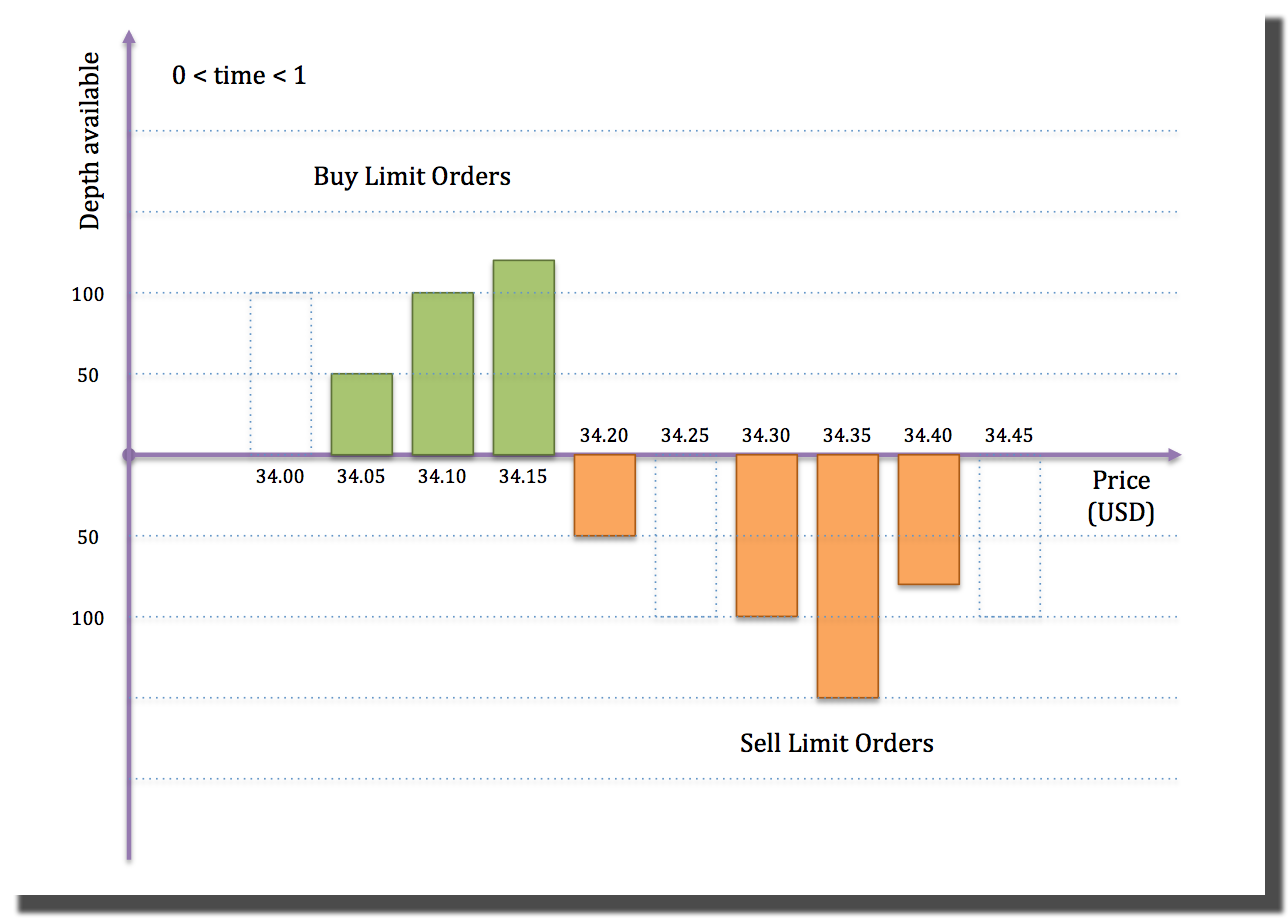
\includegraphics[height=0.9\textheight]{LOB_Match/LOB_Match_0.png}
        \caption{Limit order matching mechanism.}
        \label{fig:LOB_0}
\end{figure}
\end{frame}

% Page 10
\begin{frame}[shrink=30]{{\color{cyan}Limit order matching mechanism}}
\bigskip
\begin{figure}[H]
	\centering
	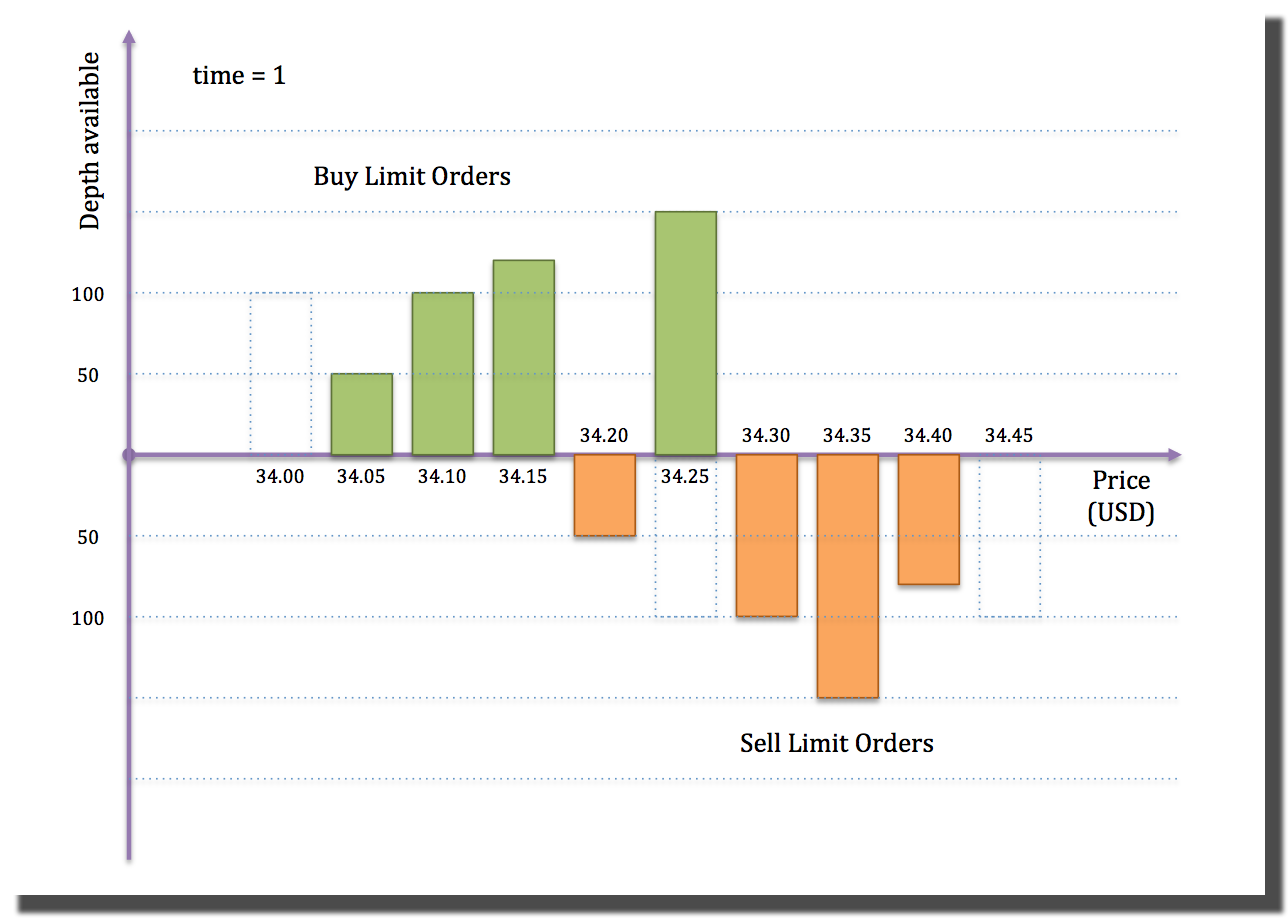
\includegraphics[height=0.9\textheight]{LOB_Match/LOB_Match_1.png}
        \caption{Limit order matching mechanism.}
        \label{fig:LOB_1}
\end{figure}
\end{frame}

% Page 11
\begin{frame}[shrink=30]{{\color{cyan}Limit order matching mechanism}}
\bigskip
\begin{figure}[H]
	\centering
	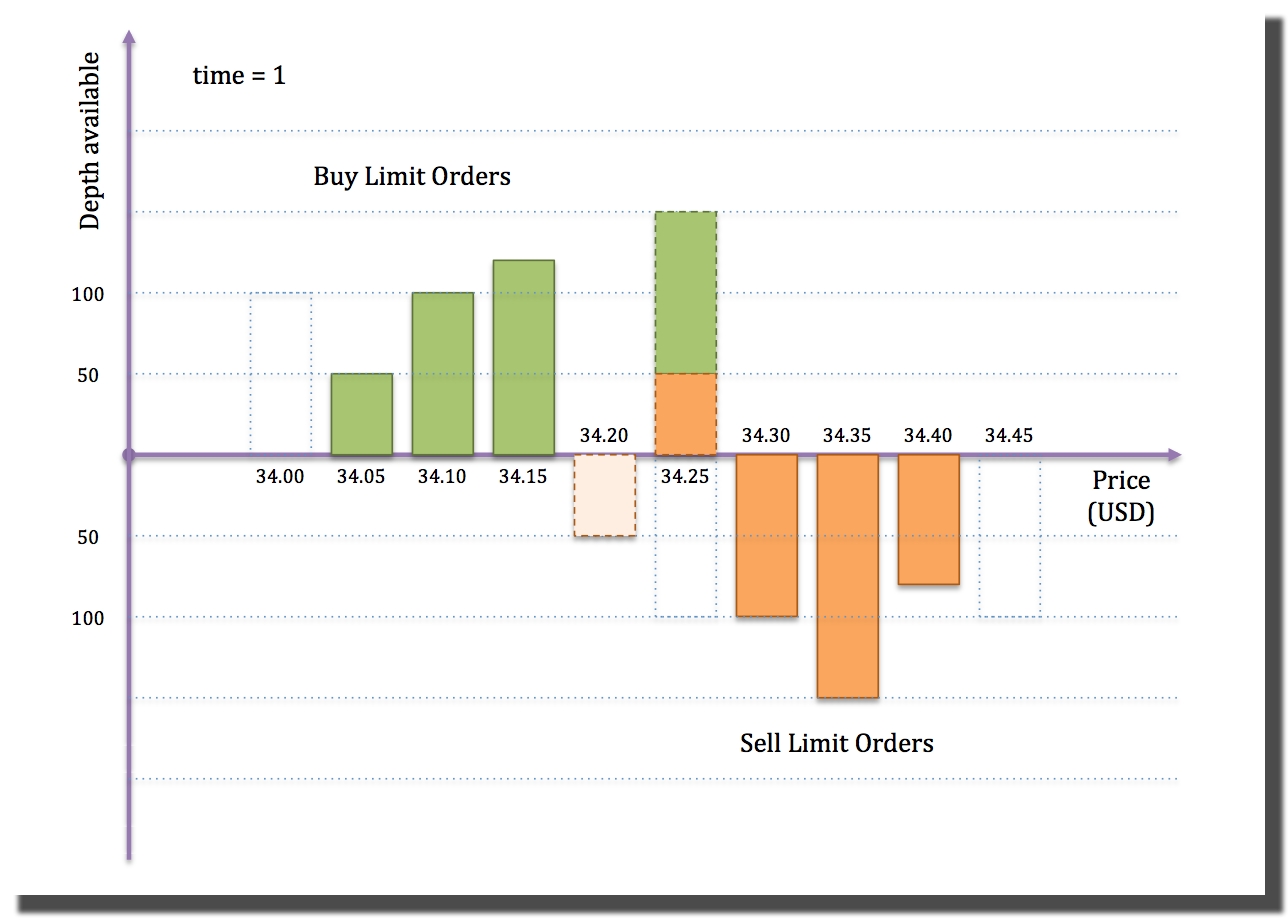
\includegraphics[height=0.9\textheight]{LOB_Match/LOB_Match_2.png}
        \caption{Limit order matching mechanism.}
        \label{fig:LOB_2}
\end{figure}
\end{frame}

% Page 12
\begin{frame}[shrink=30]{{\color{cyan}Limit order matching mechanism}}
\bigskip
\begin{figure}[H]
	\centering
	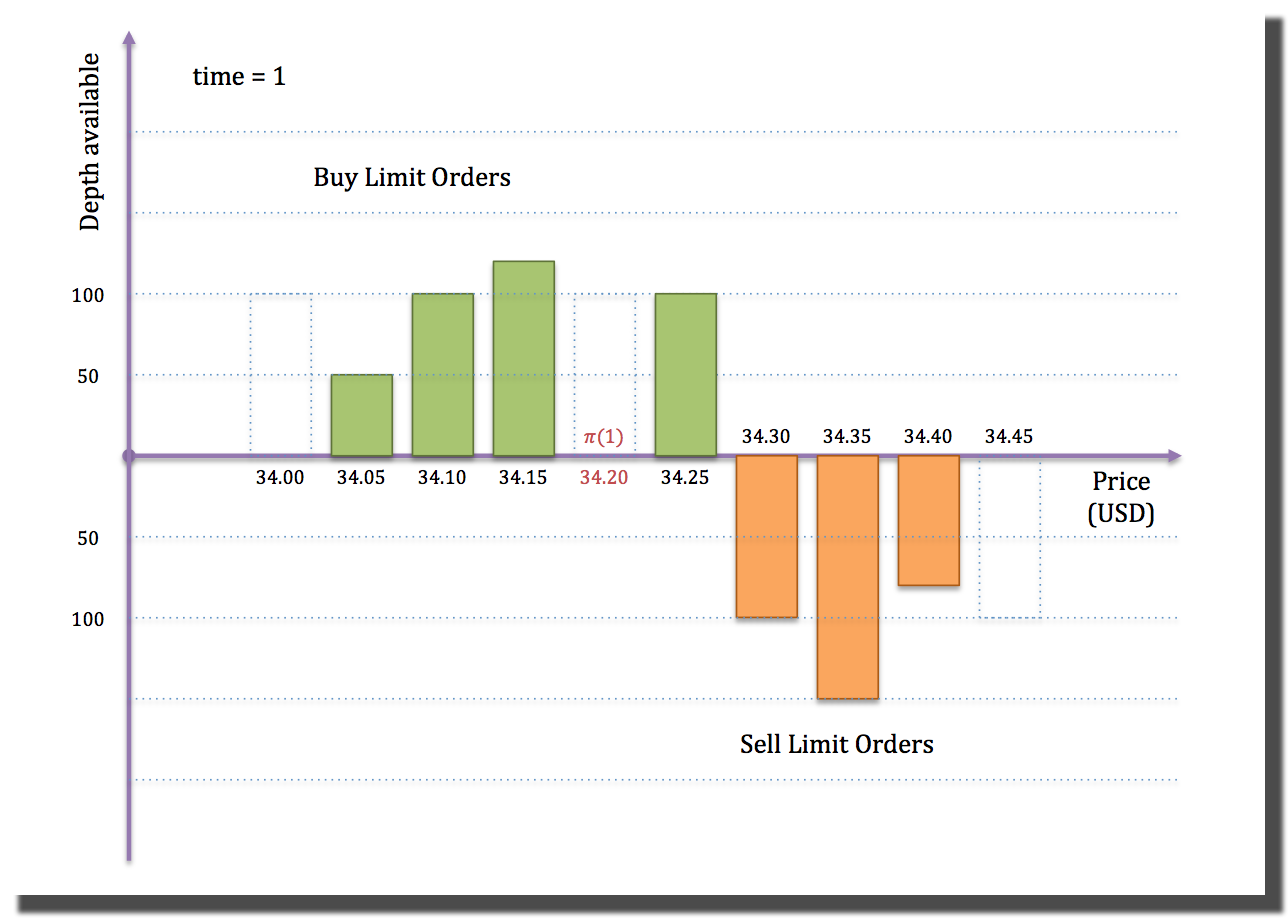
\includegraphics[height=0.9\textheight]{LOB_Match/LOB_Match_3.png}
        \caption{Limit order matching mechanism.}
        \label{fig:LOB_3}
\end{figure}
\end{frame}

% Page 13
\begin{frame}[shrink=30]{{\color{cyan}Demand v.s. Supply}}
\bigskip
The order books contain all the information about demand and supply.
\begin{figure}[htbp]
	\centering
	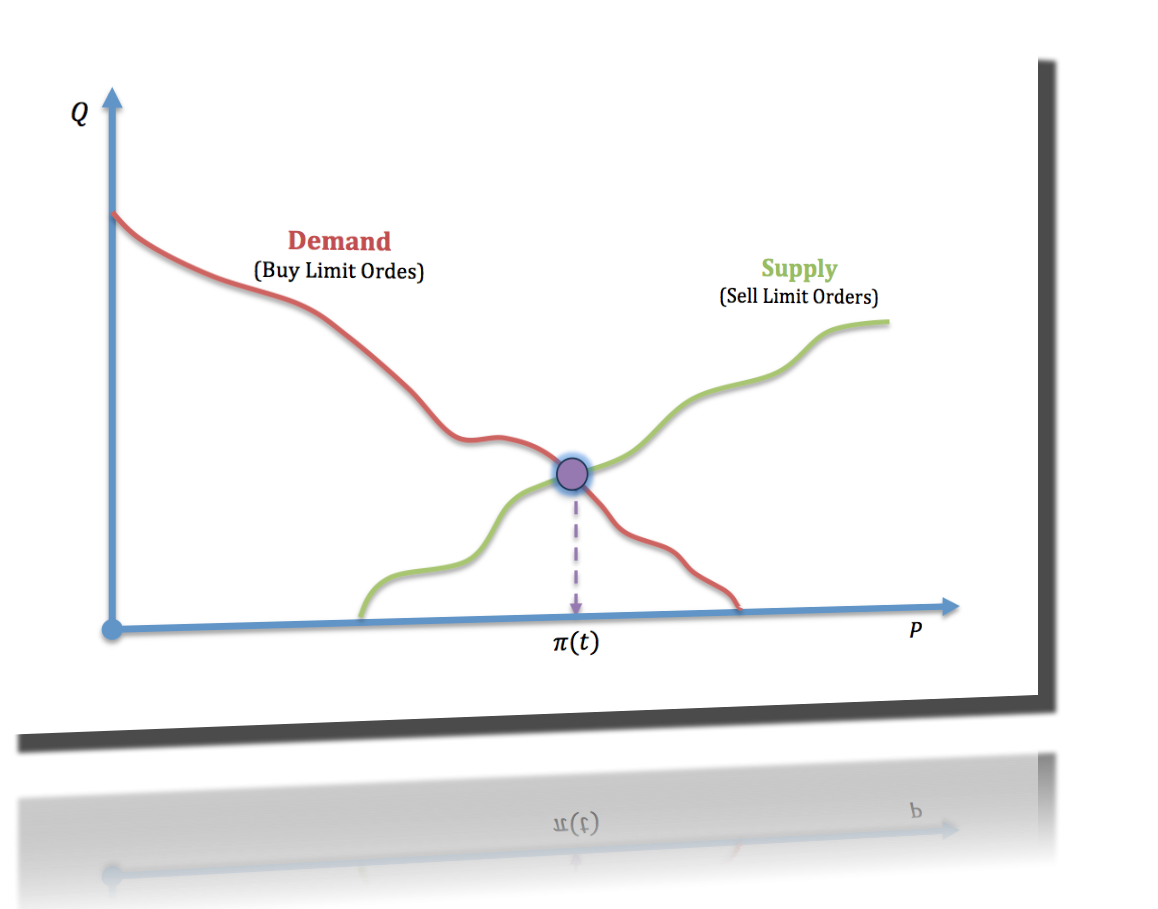
\includegraphics[height=0.9\textheight]{Demand_Supply.png}
        \caption{Demand v.s. Supply.}
        \label{fig:demand_supply}
\end{figure}

\end{frame}

% Page 14
\begin{frame}[shrink=40]{{\color{cyan}The dynamics of Limit Orders in 3D}}
\vskip 0.5in

\begin{columns}

\begin{column}{0.48\textwidth}
\begin{figure}[htbp]
                \centering
                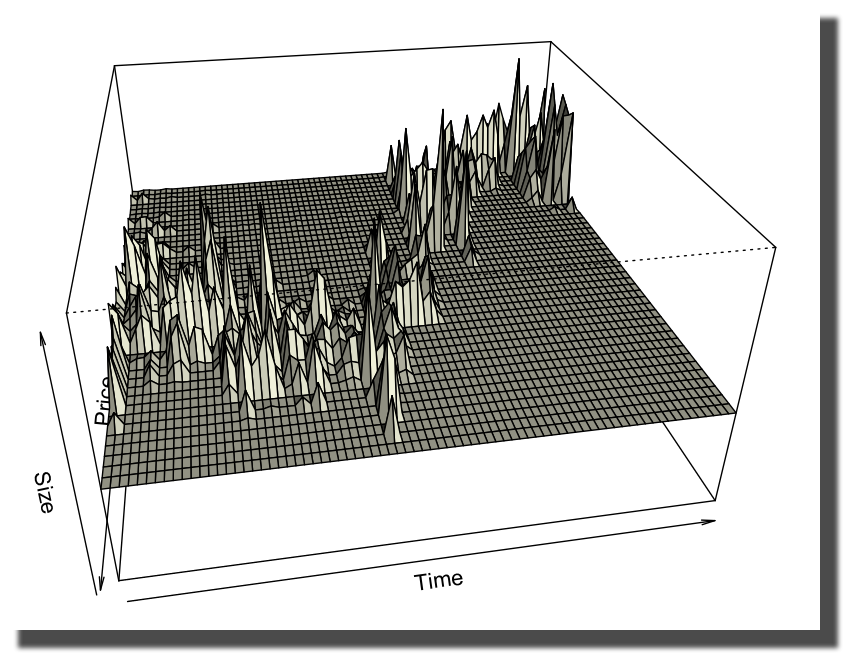
\includegraphics[width=\textwidth]{ORCL/ORCL_20110404_BuySize_3D_5min.png}
                \caption{Buy Limit Orders of ORCL on April 4, 2011.}
                \label{fig:ORCL_BuySize_3D}
\end{figure}
\end{column}

\begin{column}{0.48\textwidth}
\begin{figure}[htbp]
                \centering
                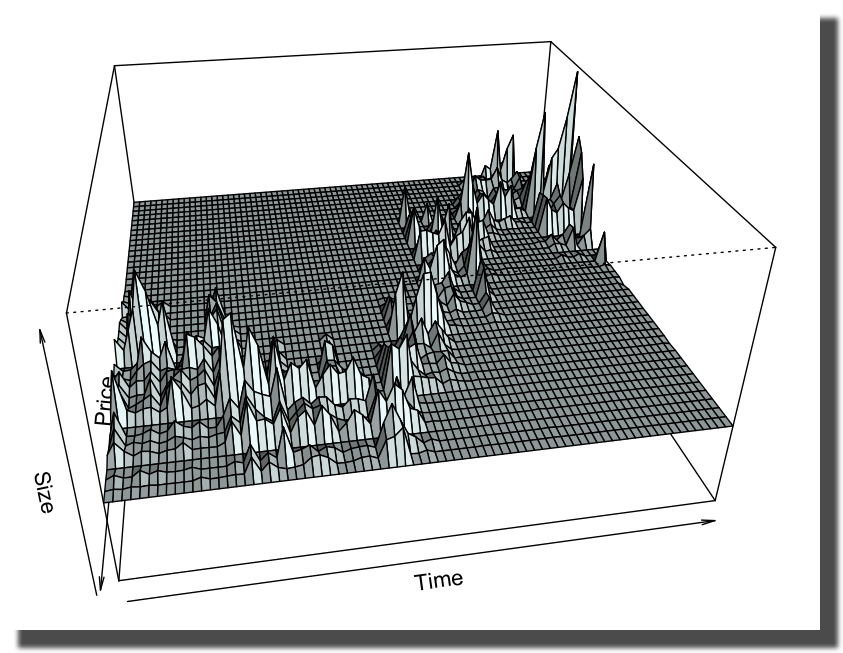
\includegraphics[width=\textwidth]{ORCL/ORCL_20110404_SellSize_3D_5min.png}
                \caption{Sell Limit Orders of ORCL on April 4, 2011.}
                \label{fig:ORCL_SellSize_3D}
\end{figure}
\end{column}

\end{columns}

\end{frame}

% Page 15
\begin{frame}[shrink=30]{{\color{cyan}The dynamics of the Clearing Price process}}
\bigskip
\begin{figure}[H]
\begin{center}
	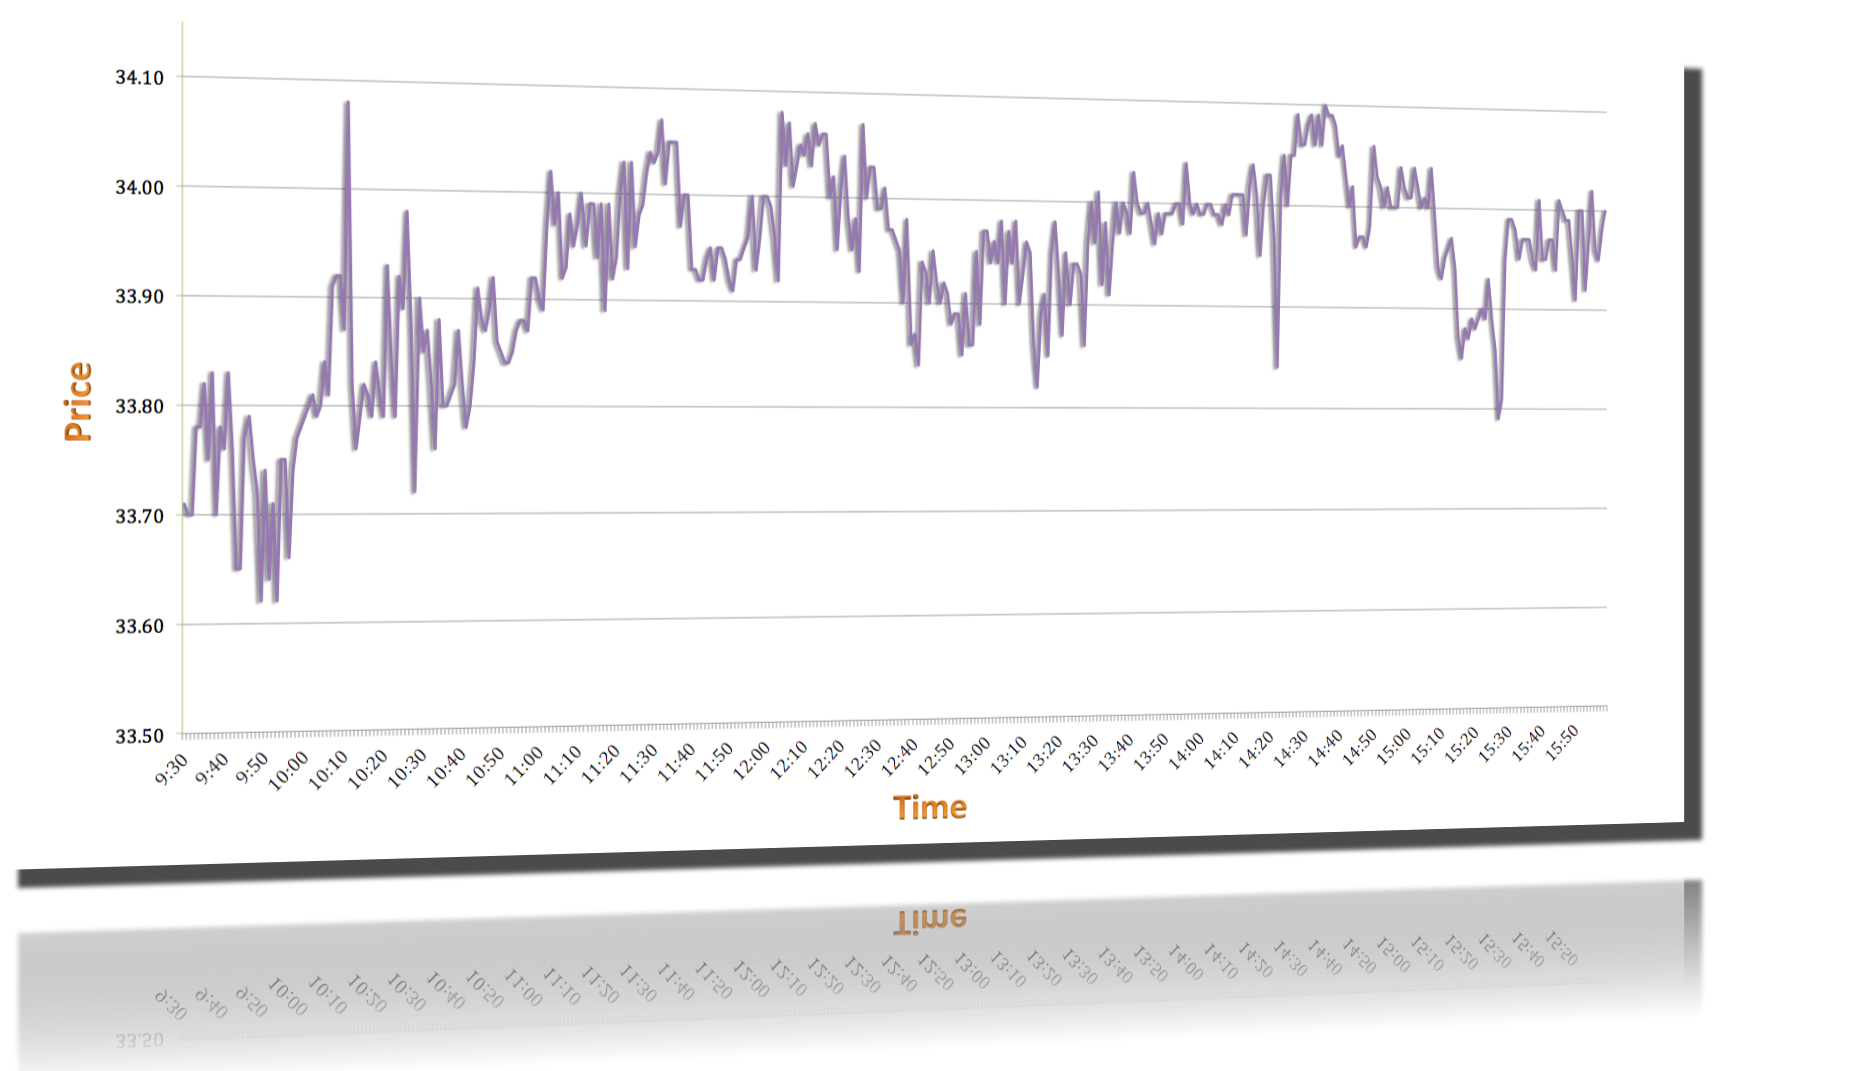
\includegraphics[height=0.9\textheight]{/ORCL/ORCL_20110401_Clearing_Prices.png}
\caption{The dynamics of Oracle Corporation's Clearing Prices on April 1, 2011.}
\label{fig:the_dynamics_ORCL_pi_20110401}
\end{center}
\end{figure}
\end{frame}

% Page 16
\begin{frame}[shrink=30]{{\color{cyan}High-Frequency Trading}}
\bigskip
\begin{figure}[H]
\begin{center}
	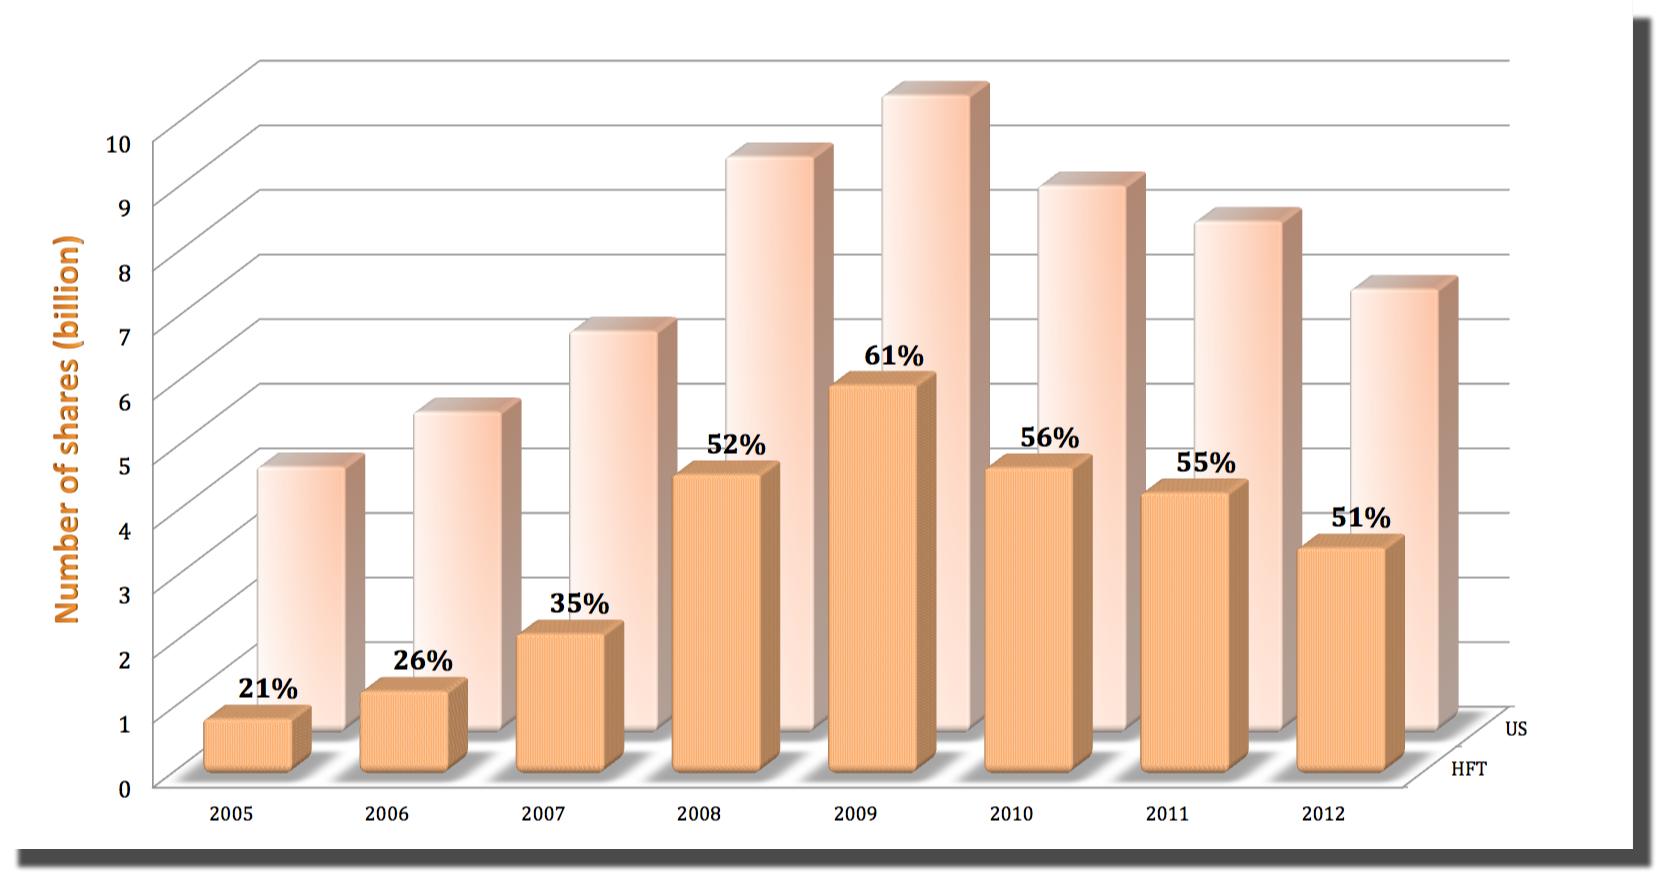
\includegraphics[height=0.9\textheight]{HFT_US_20052012.png}
\caption{Average daily trading volume by HFT firms in all U.S. stocks (2005-2012).}
\vspace{-10pt}
\caption*{{\footnotesize \textit{Source: Tabb Group, Rosenblatt Securities, The New York Times and Agarwal (2012).}}}
\label{fig:HFT_volume}
\end{center}
\end{figure}
\end{frame}

% Page 17
\section{Literature Review}
\begin{frame}[shrink=30]{{\color{cyan}Literature Review: Liquidity Models}}
\bigskip
Market Manipulation (feedback) Models
\begin{itemize}
\item Jarrow (1994),
\item Platen and Schweizer (1998),
\item Sircar and Papanicolaou (1998),
\item Frey (1998),
\item Schonbucher and Wilmott (2000),
\item Bank and Baum (2004).
\end{itemize}

\bigskip
Price-taking (competitive)\ Models
\begin{itemize}
\item Cetin, Jarrow, and Protter (2004),
\item Cetin and Rogers (2006),
\item Cetin, Soner, and Touzi (2009),
\item Kallsen and Rheinlaender (2009),
\item Gokay and Soner (2011).
\end{itemize}

\end{frame}

% Page 18
\begin{frame}[shrink=38]{{\color{cyan}Net Demand Curve and Clearing Price}}
\bigskip
\begin{block}{Definition}
The net demand curve $Q$ is a function $[0,P]\times \mathbb{R}^{+}\times \Omega \mathbb{\rightarrow R}$, which value $Q(p,t,\omega )$ is equal to the difference between the quantity of shares \textbf{available} for purchase and the quantity of shares \textbf{available} for sale at price $p$ at time $t$. For each $p$ the stochastic process $Q(.,t,)$ is a $\mathcal{F}_{t}$ adapted semimartingale.
\end{block}

{\color{magenta}\textbf{Remark:}} If we use Brownian motion to model demand, the net demand curve must be defined on a continuum of limit prices. Indeed the clearing price will be a diffusion (range = $\mathbb{R}^{+}$). Since it must fall on an existing limit price, the demand must be defined on a continuum of limit prices.

\vspace{5pt}
{\color{magenta}\textbf{Remark:}} The net demand curve should be decreasing in $p$. The easiest way to do that is to model positive processes:
\begin{itemize}
\item $Q(0,t)$: total number of buy orders
\item $q(p,t)$: density of buy orders + density of sell orders
\end{itemize}
\begin{equation*}
Q(p,t)=Q(0,t)-\int_{0}^{p}q(y,t)dy
\end{equation*}

\begin{block}{Definition}
The clearing price $\pi (t)$ is a $\mathcal{F}_{t}-$ adapted stochastic process which satisfies market clearing:
\vspace{-8pt}
\begin{equation*}
Q(\pi (t),t)=0
\end{equation*}
\end{block}

\end{frame}

\section{The Model}
% Page 19
\begin{frame}[shrink=30]{{\color{cyan}The Model}}
\bigskip
\begin{itemize}
\item It can be proved that the optimal strategy of a large trader is to disseminate her orders into infinitesimal orders.

\qquad This shows that a continuous demand curve is a plausible model.

\vspace{10pt}
\item For the clearing price to be a martingale, it is (generically) necessary to have as many "sources of information" as possible limit price values:

\qquad since the set of possible limit price values has to be a continuous range we introduce the Brownian sheet $W(t,s)$.

\vspace{10pt}
\item There is correlation among net demand at different limit prices
\end{itemize}

\vspace{-20pt}
\begin{align*}
dQ(0,t) &=\mu _{Q}(0,t)dt-\sigma _{Q}(0,t)\int_{s}b_{q}(0,s,t)W(0,dt), \qquad Q(0,0)=Q_{0}(0) \\
dq(p,t) &=\mu _{q}(p,t)dt+\sigma _{q}(p,t)\int_{s}b_{q}(p,s,t)W(ds,dt), \qquad q(p,0)=Q_{0}(p)\text{ \ for }0<p\leq S \\
q(0,t) &=0
\end{align*}

\end{frame}

% Page 20
\section{Main Result}
\begin{frame}[shrink=30]{{\color{cyan}Main Result: Market with a Large Trader}}
\bigskip
\begin{block}{Main Result}
\emph{Suppose in addition to our standing assumptions that

C1) for self-financing strategies involving only immediate orders, (Jarrow, 1994)'s discrete-time conditions for absence of market manipulation strategy hold,

C2) no arbitrage strategy involves wait orders,

C3) the volatility $\sigma _{Q_{A}}(p,t)$ is bounded away from zero,
uniformly in $p$,

C4) there is no path such that $Q(S,t)\geq 0$ or $Q(0,t)\leq 0$.

\vskip 0.1in
\noindent Then

F1) there exists at least one martingale measure $\mathbb{Q}$ for $\int L_L(\vartheta ,dt)$,

F2) there is no arbitrage strategy,

F3) the net demand curve $Q$ is continuous in $t$,

F4) the clearing price $\pi (t)$ is continuous,

{\color{red}F5) any such measure $\mathbb{Q}$ is also a martingale measure for $\pi (t)$}.}
\end{block}

\end{frame}

% Page 21
\begin{frame}[shrink=30]{{\color{cyan}Characterization of the Risk-Neutral Measure $\mathbb{Q}$}}
\bigskip
{\color{magenta}\textbf{Standing assumption:}} There is no path such that $Q(P,t)\geq 0$

\bigskip
\begin{block}{Change of Measure}
In the $\mathbb{Q}$-measure the process $W^{\mathbb{Q}}$ is a Brownian sheet, where:
\begin{equation*}
W^{\mathbb{Q}}(ds,dt)=W(ds,dt)+\lambda (s,t)dt
\end{equation*}

\textbf{Goal:} determine $\lambda $ such that $\pi $ is a $\mathbb{Q}$-martingale.
\end{block}

\end{frame}

% Page 22
\section{Market Price of Risk Equations}
\begin{frame}[shrink=30]{{\color{cyan}Market Price of Risk Equations}}
\bigskip
Define
\begin{eqnarray*}
C(\pi ,t) &=&-\sigma _{\pi }(t)\left( \frac{\partial }{\partial p}\left(\sigma _{q}(0,t)\int_{s}b_{q}(0,s,t)b_{\pi }(s,t)ds\right) +\sigma _{q}(\pi,t)\int_{s}b_{q}(\pi ,s,t)b_{\pi }(s,t)ds\right),  \\
b(\pi ,t) &=&-\mu _{Q}(0,t)+\int_{0}^{\pi }\mu _{q}(p,t)dpdt+\frac{1}{2}\frac{\partial q}{\partial p}(\pi ,t)(\sigma _{\pi }(t))^{2}-C(\pi ,t), \\
\Sigma (\pi ,s,t) &=&\int_{0}^{\pi }\sigma _{q}(p,t)b_{q}(p,s,t)ds.
\end{eqnarray*}

\bigskip
The market price of risk equations are:
\begin{equation*}
\int_{s=0}^{P}\Sigma (\pi ,s,t)\lambda (s,t)ds=b(\pi ,t)\text{ \ \ \ \ \ } 0\leq \pi \leq P
\end{equation*}

\begin{block}{Theorem}
Suppose all the previous assumptions hold. In addition, suppose that the market price of risk equations have a unique solution. Then there is no arbitrage.
\end{block}

\end{frame}

% Page 23
\begin{frame}[shrink=30]{{\color{cyan}From a "MetaModel" to a Model}}
\bigskip
Reminder:
\begin{eqnarray*}
q(p,t)dp &=&\text{sum of buy and sell order quantities with limit price} \\
&&\text{in }[p,p+dp]\text{ arriving in }[0,t]\text{ }
\end{eqnarray*}

Plausible dynamics for $q$:

\begin{itemize}
\item positive process

\qquad \qquad not necessarily increasing: orders can be cancelled

\item mean-reverting process

\item to be implemented on a computer: $p$ and $t$ must take discrete values

\item the relative curve, i.e., the two-argument curve $\tilde{q}(.,.,t)$
where $\tilde{q}(p-\pi (t),p,t)=q(p,t)$ can be well fitted as a function of
the first argument only
\end{itemize}

{\color{magenta}\textbf{Our choice:}} the exponential of a (vector) Ornstein-Uhlenbeck process.

\end{frame}

% Page 24
\section{Empirical Analysis}
\begin{frame}[shrink=35]{{\color{cyan}NYSE Arcabook Data}}
\bigskip
\begin{table}[H]
\begin{center}
\begin{tabular}{llll}
\hline
\textbf{Industry} & \textbf{Exchange} & \textbf{Ticker} & \textbf{Firm}\\
\hline \hline

\multirow{2}{*}{Energy} & NYSE & CVX & Chevron Corporation\\
 & NYSE & XOM & Exxon Mobil Corporation\\

\hline
\multirow{2}{*}{Financial Banks} & NYSE & JPM & JPMorgan Chase \& Co.\\
 & NYSE & WFC & Wells Fargo \& Company \\

 \hline
 \multirow{2}{*}{Materials and Mining} & NYSE & ABX & Barrick Gold Corporation \\
 & NYSE & FCX & Freeport-McMoRan Copper \& Gold Inc. \\

 \hline
 \multirow{3}{*}{Technology} & NASDAQ & CSCO & Cisco Systems, Inc. \\
 & NASDAQ & MSFT & Microsoft Corporation \\
 & NASDAQ & ORCL & Oracle Corporation \\
\hline
\end{tabular}
\end{center}
\caption{NYSE Arcabook data selection.}
\label{table:NYSE_Arcabook_Selection}
\end{table}

\end{frame}

% Page 25
\begin{frame}[shrink=35]{{\color{cyan}Parameter Estimation}}
\bigskip
\begin{figure}[htbp]
                \centering
                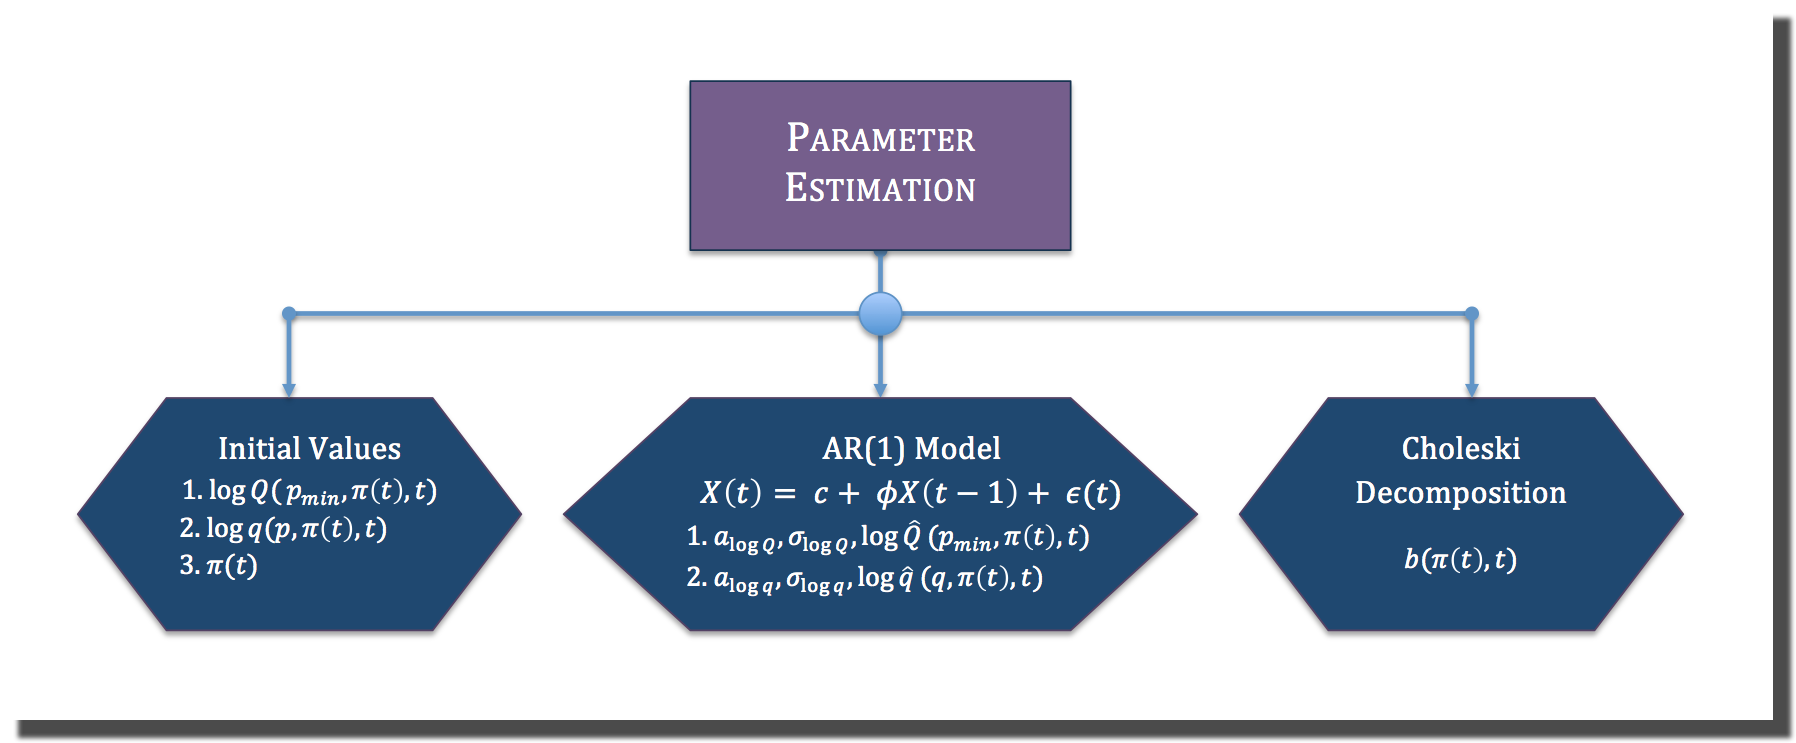
\includegraphics[width=0.9\textwidth]{Parameter_Estimation.png}
                \caption{Parameter Estimation}
                \label{fig:parameter_estimation}
\end{figure}

\end{frame}

% Page 26
\begin{frame}[shrink=50]{{\color{cyan}Volatility Smile ({\color{magenta}ORCL})}}
\bigskip
\begin{columns}

\begin{column}{0.3\textwidth}
\begin{table}[H]
\begin{center}
\begin{tabular}{cc}
\hline
\textbf{Strike Price}	& \textbf{Implied Volatility}\\
\hline \hline
33.77	& 22.66\%\\
33.80	& 21.05\%\\
33.83	& 19.40\%\\
33.87	& 17.71\%\\
33.90	& 15.94\%\\
33.93	& 14.10\%\\
33.97	& 12.16\%\\
34.00	& 10.11\%\\
{\color{orange}34.04}	& 9.35\%\\
34.07	& 10.26\%\\
34.10	& 11.03\%\\
34.14	& 11.70\%\\
34.17	& 12.25\%\\
34.20	& 12.71\%\\
34.24	& 13.06\%\\
34.27	& 13.25\%\\
34.31	& 13.34\%\\
34.34	& 13.32\%\\
34.37	& 13.23\%\\
34.41	& 12.99\%\\
\hline
\end{tabular}
\label{tab:ORCL_volatility_smile}
\end{center}
\end{table}
\end{column}

\begin{column}{0.7\textwidth}
\begin{figure}[htbp]
                \centering
                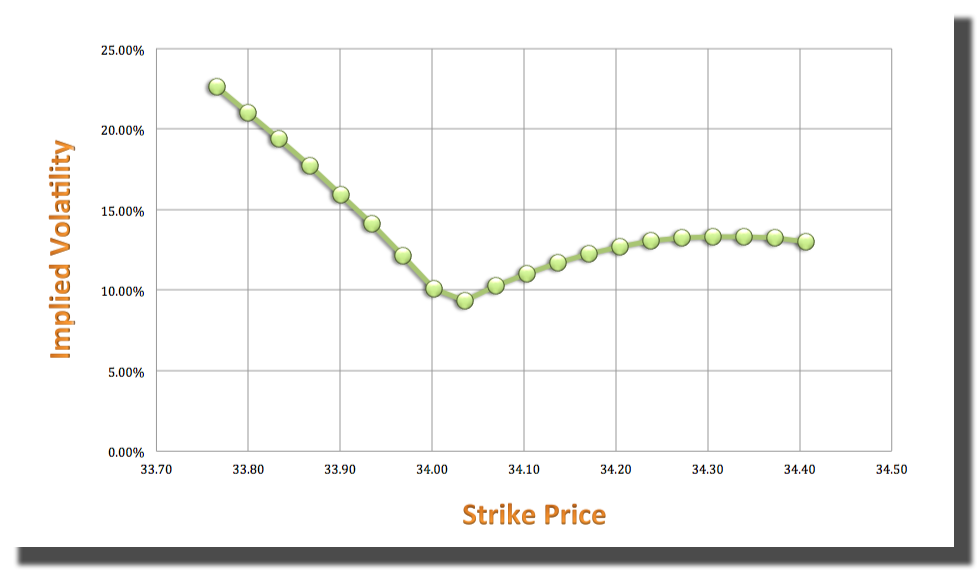
\includegraphics[height=0.75\textheight]{ORCL/ORCL_20110404_Simulated_Volatility_Smile.png}\\
                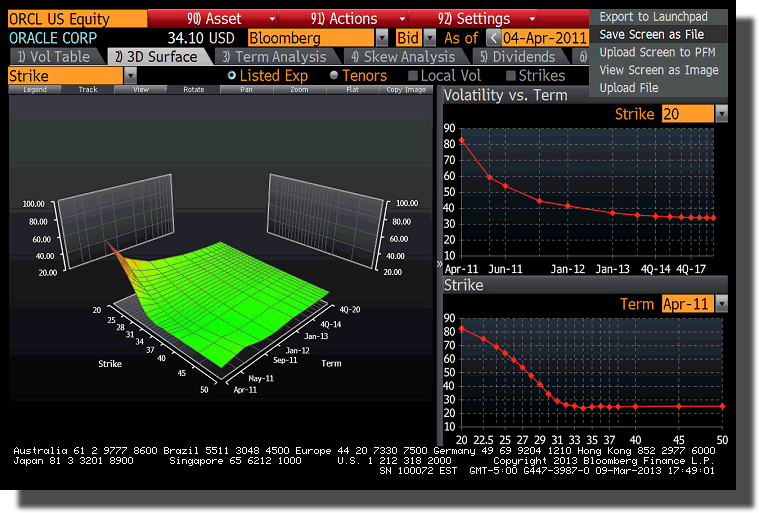
\includegraphics[height=0.75\textheight]{ORCL/ORCL_20110404_B.png}\\
                \caption{Simulated v.s. real-time volatility smile of ORCL on April 4, 2011. \textit{Source: Bloomberg}}
                \label{fig:ORCL_VolSmile_SimvsReal}
\end{figure}
\end{column}
\end{columns}

\end{frame}

% Page 27
\begin{frame}[shrink=50]{{\color{cyan}Volatility Smile ({\color{magenta}ABX})}}
\bigskip
\begin{columns}

\begin{column}{0.3\textwidth}
\begin{table}[H]
\begin{center}
\begin{tabular}{cc}
\hline
\textbf{Strike Price}	& \textbf{Implied Volatility}\\
\hline \hline
50.98	& 23.64\%\\
51.03	& 21.98\%\\
51.08	& 20.27\%\\
51.13	& 18.51\%\\
51.18	& 16.70\%\\
51.23	& 14.84\%\\
51.29	& 12.93\%\\
{\color{orange}51.34}	& 11.69\%\\
51.39	& 12.24\%\\
51.44	& 12.75\%\\
51.49	& 13.20\%\\
51.54	& 13.58\%\\
51.59	& 13.92\%\\
51.64	& 14.18\%\\
51.69	& 14.37\%\\
51.74	& 14.46\%\\
51.79	& 14.54\%\\
51.85	& 14.55\%\\
51.90	& 14.46\%\\
51.95	& 14.39\%\\
\hline
\end{tabular}
\label{tab:ABX_volatility_smile}
\end{center}
\end{table}
\end{column}

\begin{column}{0.7\textwidth}
\begin{figure}[htbp]
                \centering
                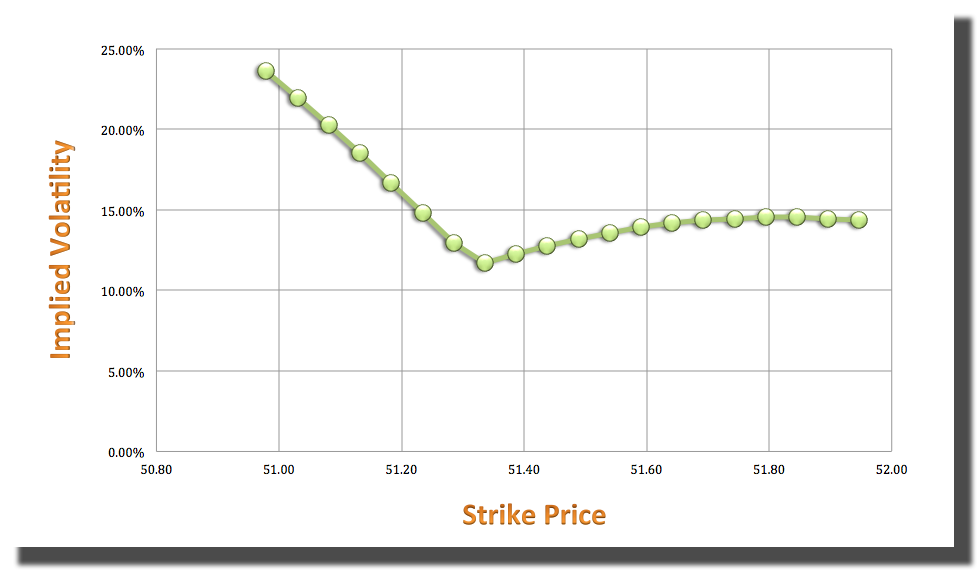
\includegraphics[height=0.75\textheight]{ABX/ABX_20110404_Simulated_Volatility_Smile.png}\\
                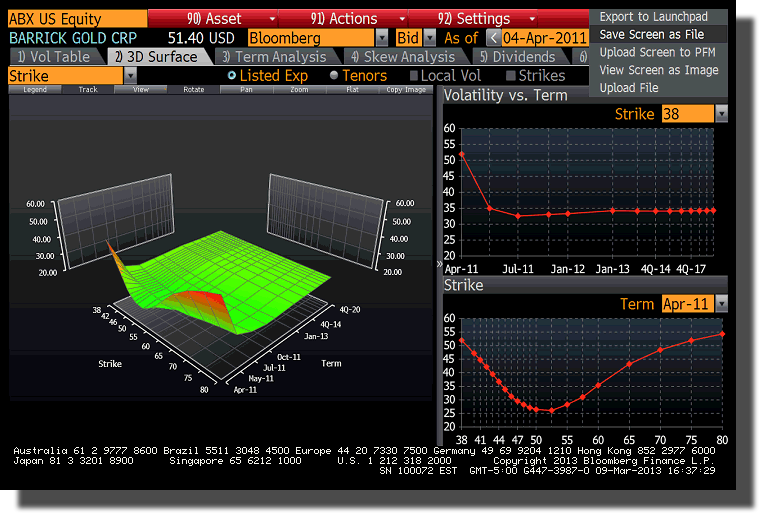
\includegraphics[height=0.75\textheight]{ABX/ABX_20110404_B.png}\\
                \caption{Simulated v.s. real-time volatility smile of ABX on April 4, 2011. \textit{Source: Bloomberg}}
                \label{fig:ABX_VolSmile_SimvsReal}
\end{figure}
\end{column}
\end{columns}

\end{frame}

% Page 28
\begin{frame}[shrink=50]{{\color{cyan}Volatility Smile ({\color{magenta}CSCO})}}
\bigskip
\begin{columns}

\begin{column}{0.3\textwidth}
\begin{table}[H]
\begin{center}
\begin{tabular}{cc}
\hline
\textbf{Strike Price}	& \textbf{Implied Volatility}\\
\hline \hline
16.88	& 13.30\%\\
16.90	& 12.17\%\\
16.92	& 11.02\%\\
16.93	& 9.84\%\\
16.95	& 8.63\%\\
16.97	& 7.37\%\\
16.99	& 6.04\%\\
17.00	& 4.63\%\\
{\color{orange}17.02}	& 4.16\%\\
17.04	& 4.84\%\\
17.05	& 5.28\%\\
17.07	& 5.53\%\\
17.09	& 5.68\%\\
17.10	& 5.73\%\\
17.12	& 5.79\%\\
17.14	& 5.85\%\\
\hline
\end{tabular}
\label{tab:CSCO_volatility_smile}
\end{center}
\end{table}
\end{column}

\begin{column}{0.7\textwidth}
\begin{figure}[htbp]
                \centering
                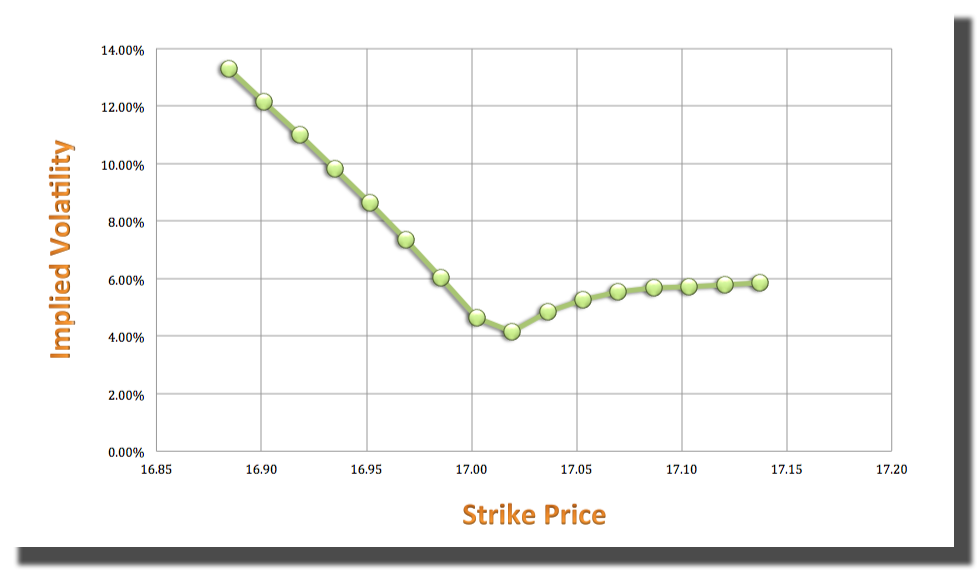
\includegraphics[height=0.75\textheight]{CSCO/CSCO_20110404_Simulated_Volatility_Smile.png}\\
                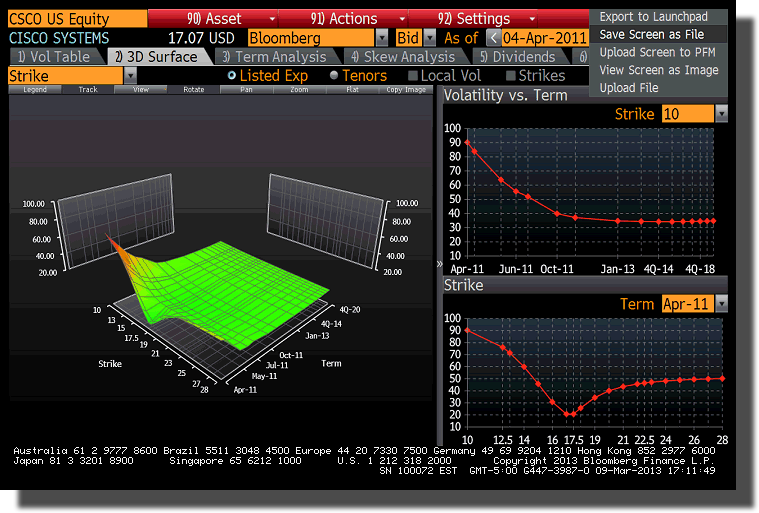
\includegraphics[height=0.75\textheight]{CSCO/CSCO_20110404_B.png}\\
                \caption{Simulated v.s. real-time volatility smile of CSCO on April 4, 2011. \textit{Source: Bloomberg}}
                \label{fig:CSCO_VolSmile_SimvsReal}
\end{figure}
\end{column}
\end{columns}

\end{frame}

%%%%%%%%%%%%%%%%%%%%%%%%%%%%%%%
\section{Conclusions}

% Page 29
\begin{frame}[shrink=25]{{\color{cyan}Conclusions}}
\bigskip
\begin{enumerate}
\item We developed a liquidity model with stands between
		\begin{itemize}
			\item traditional no-arbitrage (option pricing)\ models and
			\item financial economics models.
		\end{itemize}

\vspace{5pt}
\item This model uses Ito-Wentzell's formula and Girsanov's theorem for Brownian sheets.

\vspace{5pt}
\item We give conditions for no-arbitrage, which allows us to price options

\vspace{5pt}
\item We specified a model
		\begin{itemize}
			\item with positive demand density,
			\item with mean-reversion,
			\item where parameters are centered on the clearing price.
		\end{itemize}

\vspace{5pt}	
\item The model generates an implied volatility smile which matches the observed smile much better than the traditional Black-Scholes model.

\end{enumerate}
\end{frame}

% Page 30
\begin{frame}[shrink=25]{{\color{cyan}Conclusions}}
\bigskip

Thank you!

\end{frame}

\end{document}
%%%%%%%%%%%%%%%%%%%%%%%%%%%%%% 